% !TEX program = xelatex
\documentclass[12pt, a4paper]{article}
\input{packages.tex}
% 設定頁面邊距
\geometry{
    a4paper,
    left=1cm,
    right=1cm,
    top=2cm,
    bottom=2cm
}

\hypersetup{hidelinks}
\setlength{\headheight}{14.5pt}

% 允許 TeX 在必要時提早折行（吸收少量過長行），避免文字溢出右邊界。
\emergencystretch=3em

% 設定字型
\setmainfont[
    Path = ./fonts/Times_New_Roman/,
    BoldFont = *-bold,
    ItalicFont = *-italic,
    BoldItalicFont = *-bold_italic
]{times}

\setmonofont[
    Path = ./fonts/Roboto_Mono/static/,
    UprightFont = *-Regular,
    BoldFont = *-Bold,
    ItalicFont = *-Italic,
    BoldItalicFont = *-BoldItalic
]{RobotoMono}

\xeCJKsetup{AutoFakeBold=true, AutoFakeSlant=true}
\setCJKmainfont[
    Path = ./fonts/kaiu/,
]{kaiu}
\setCJKmonofont{./fonts/kaiu/kaiu.ttf}

% 頁面設定
\fancyhf{}
\rfoot{\thepage}

% 設置圖片路徑
\graphicspath{{fig/}}

% 標題樣式
\titleformat{\section}{\large\bfseries}{\thesection}{1em}{}
\titleformat{\subsection}{\normalsize\bfseries}{\thesubsection}{1em}{}


\pagestyle{fancy}
\fancyhf{}
\rhead{June. 2026}
\lhead{\textbf{Visual Recognition using Deep Learning
2026 Spring}}
\rfoot{\thepage}


\begin{document}

% \maketitle
\begin{center}
    \LARGE \textbf{HuBMAP - Hacking the Human Vasculature}\\[0.4em]
    \large 535521 Selected Topics in Visual Recognition using Deep Learning\\
    \large 徐葆驊、吳念澤、江怜儀、王妤瑄\\
    \normalsize Group14\\
    \vspace{0.5em}
    \normalsize GitHub: \url{https://github.com/benhsu0828/2026version_HuBMAP_Hacking_the_Human_Vasculature.git}
\end{center}

\vspace{1em}

\begingroup
\footnotesize

\section{Introduction}
\label{sec:intro}

This project studies the Kaggle competition \textit{HuBMAP -- Hacking the Human Vasculature}~\cite{hubmap2023}. The task is instance segmentation: for each $512 \times 512$ histology tile, the model must output separate object masks with confidence scores. The final evaluation follows a mean Average Precision (mAP) style metric over instance masks, so both localization quality and mask quality matter.

The training data is heterogeneous. Dataset 1 contains the cleanest annotations and is used as the main validation and fine-tuning source in our experiments. Dataset 2 contains more weak/noisy annotations and is useful for increasing data coverage, but it can also inject label noise. Dataset 3 provides additional whole-slide image (WSI) regions; in our implementation it is treated mainly as extra WSI context in the dataset metadata, while the main training pipelines focus on Dataset 1 and Dataset 2. This setting makes cross-validation design important: neighboring tiles from the same WSI can be visually similar, so random tile-level splits would overestimate generalization.

\section{Methodology and related work}
\label{sec:top}

First we survey the top Kaggle solutions and identify key design choices. Here are the main models and techniques that influenced our implementation.

\subsection{First-place models}

\begin{itemize}
    \item \textbf{RTMDet}~\cite{rtmdet} is a real-time one-stage detector built from a CSPNeXt backbone and a CSPNeXt-PAFPN neck, trained with a dynamic soft-label assigner. The first place uses the largest variant, RTMDet-X, as its best single model and bolts an FCN mask head on top so the same network can be supervised with masks.
    \item \textbf{YOLOX}~\cite{yolox} is an anchor-free member of the YOLO family with a decoupled detection head and SimOTA label assignment. The first place uses YOLOX-X, again augmented with mask supervision, as one ensemble stream.
    \item \textbf{Mask R-CNN}~\cite{maskrcnn} is the canonical two-stage instance segmentor: it extends Faster R-CNN with RoIAlign and a parallel FCN mask branch. In the first-place ensemble the Mask R-CNN stream uses a \textbf{Swin Transformer}~\cite{swin} backbone, a hierarchical vision transformer with shifted-window self-attention, and its mask head re-predicts the final ensemble masks at input size $1440$.
    \item \textbf{Weighted Boxes Fusion (WBF)}~\cite{wbf} is the box-level ensembling step that merges overlapping boxes from all streams by confidence-weighted averaging, rather than discarding them as NMS would.
\end{itemize}

\subsection{Third-place models}

\begin{itemize}
    \item \textbf{ViT-Adapter}~\cite{vitadapter} injects spatial priors into a plain pretrained Vision Transformer through a lightweight adapter, letting a strong ViT backbone perform dense prediction. The third place uses the large variant (ViT-Adapter-L) as its highest-scoring backbone.
    \item \textbf{CBNetV2}~\cite{cbnetv2} is a composite-backbone design that links several (here Swin-based) backbones through composite connections to form a higher-capacity feature extractor without training from scratch.
    \item \textbf{DetectoRS}~\cite{detectors} combines a Recursive Feature Pyramid with Switchable Atrous Convolution. In the third place it is paired with the \textbf{Hybrid Task Cascade (HTC)}~\cite{htc} head, which interleaves box and mask prediction across cascade stages, on \textbf{ResNeXt-101}~\cite{resnext} and \textbf{ResNet-50}~\cite{resnet} backbones to add CNN-style diversity to the transformer models.
\end{itemize}

\subsection{Our models}

\begin{itemize}
    \item \textbf{YOLO26x-Seg}~\cite{ultralytics} is the segmentation variant of Ultralytics' anchor-free single-stage YOLO detector. We used the largest (\texttt{x}) configuration to obtain an architecturally different stream from the Cascade/Mask R-CNN family.
    \item \textbf{InternImage-T}~\cite{internimage} is a CNN-based vision foundation backbone whose core operator is the DCNv3 deformable convolution; \texttt{T} denotes the tiny variant. We run the pure-PyTorch \texttt{DCNv3\_pytorch} operator so the model needs no custom CUDA compilation, which makes it easy to package for Kaggle.
    \item \textbf{Cascade Mask R-CNN}~\cite{cascade_rcnn,maskrcnn} extends Mask R-CNN with a multi-stage cascade of detection heads trained at increasing IoU thresholds, which progressively refines box quality; we attach an FCN mask head and a \textbf{Feature Pyramid Network (FPN)}~\cite{fpn} neck for multi-scale fusion.
\end{itemize}

\subsection{First-place direction: WSI-aware heterogeneous ensembles}

The first-place Kaggle write-up frames the problem as box-quality-driven instance segmentation: AP is dominated by bounding-box localization, while mask prediction can be delegated to a strong mask head after the boxes are fixed~\cite{tascj2023hubmapfirst}. This explains why the public release is not a single semantic-segmentation model. It is a heterogeneous MMDetection ensemble that includes RTMDet-X, YOLOX-X, and Mask R-CNN streams. The released training repository also marks RTMDet-X as the best single model, and its configs add mask supervision through an extra mask head on top of the detector~\cite{tascj2023hubmapfirst}.

Several design choices are especially relevant:
\begin{itemize}
    \item \textbf{WSI-aware validation using two of five spatial folds.} The first place does not use a full $k$-fold cross-validation ensemble. The write-up states that every model is trained with ``two different weights (2 of 5 folds)'', and the released \texttt{tools/\allowbreak prepare\_\allowbreak data.py} ships exactly those two folds. Tiles from the clean Dataset 1 of WSI 1 and WSI 2 are sorted by their vertical tile index \texttt{i} and conceptually divided into five contiguous 20\% bands. Fold 0 holds out the lowest band ($\texttt{i}<$ the 20th percentile) as validation (\texttt{dval0i}) and trains on the rest (\texttt{dtrain0i}); fold 1 holds out the highest band ($\texttt{i}>$ the 80th percentile, \texttt{dval1i}/\texttt{dtrain1i}). Because each validation set is a contiguous spatial band instead of randomly sampled tiles, neighboring tiles from the same WSI cannot leak between train and validation. The author reports this split as harder but more trustworthy than random splitting: about $0.47$ bbox / $0.72$ segm mAP@60 under random splitting versus $0.43$ / $0.68$ under the \texttt{i} split.
    \item \textbf{EMA as a stabilizer.} The author highlights Exponential Moving Average (EMA) as the most important technique in the experiments. Multiple EMA copies were evaluated from a single training run, which gave a stable basis for model selection.
    \item \textbf{Mask supervision for better boxes.} RTMDet-X already produced strong boxes, but adding mask supervision and random rotation improved bbox mAP. The mask head was therefore used not only for final masks, but also as an auxiliary signal for localization.
    \item \textbf{Box-first ensemble.} The final ensemble uses WBF over three RTMDet models, one YOLOX-X model with mask supervision, and one Mask R-CNN. All five model types are represented by two different fold weights. The final masks are generated from a Mask R-CNN mask head at input size 1440, and the write-up explicitly notes that no TTA was used.
\end{itemize}

The role of the two folds is therefore not mainly variance estimation; it is a cheap two-member bagging ensemble. In the released configs each of the five model families is trained once per fold: \texttt{r}, \texttt{s}, and \texttt{sb} are all RTMDet-with-mask variants (three RTMDet streams), \texttt{y} is YOLOX-X with mask supervision, and \texttt{m} is a Swin-backbone Mask R-CNN. Training each family on both folds yields the ten inference streams $\{\texttt{r},\texttt{s},\texttt{m},\texttt{y},\texttt{sb}\}\times\{\texttt{0i},\texttt{1i}\}$ that the ensemble fuses, so every test tile is processed by two independently held-out weight sets of every architecture. This is also why our YOLO extension below adds its own four spatial folds: it follows the same fold-as-bagging philosophy, just with more members.

This project therefore uses the first-place pipeline as the main baseline: reproduce the MMDetection ensemble behavior, keep the bbox-first interpretation of the metric, then test whether a new stream improves or hurts the fused box set.

\subsection{Third-place direction: multi-stage training}

The third-place write-up focuses on how to properly use noisy annotations~\cite{nischay2023hubmapthird}. The final system uses five MMDetection-based models: two ViT-Adapter-L models, one CBNetV2-Base model, one DetectoRS ResNeXt-101-32x4d model, and one DetectoRS ResNet-50 model. The author reports using only competition data, with no external image data. The key training idea is multi-stage learning: first pretrain on all noisy Dataset 2 WSIs for a short schedule with light augmentation and high learning rate, then fine-tune on clean Dataset 1 for more epochs with heavier augmentation, higher image resolution, and a lower learning rate.

\begin{figure}[H]
    \centering
    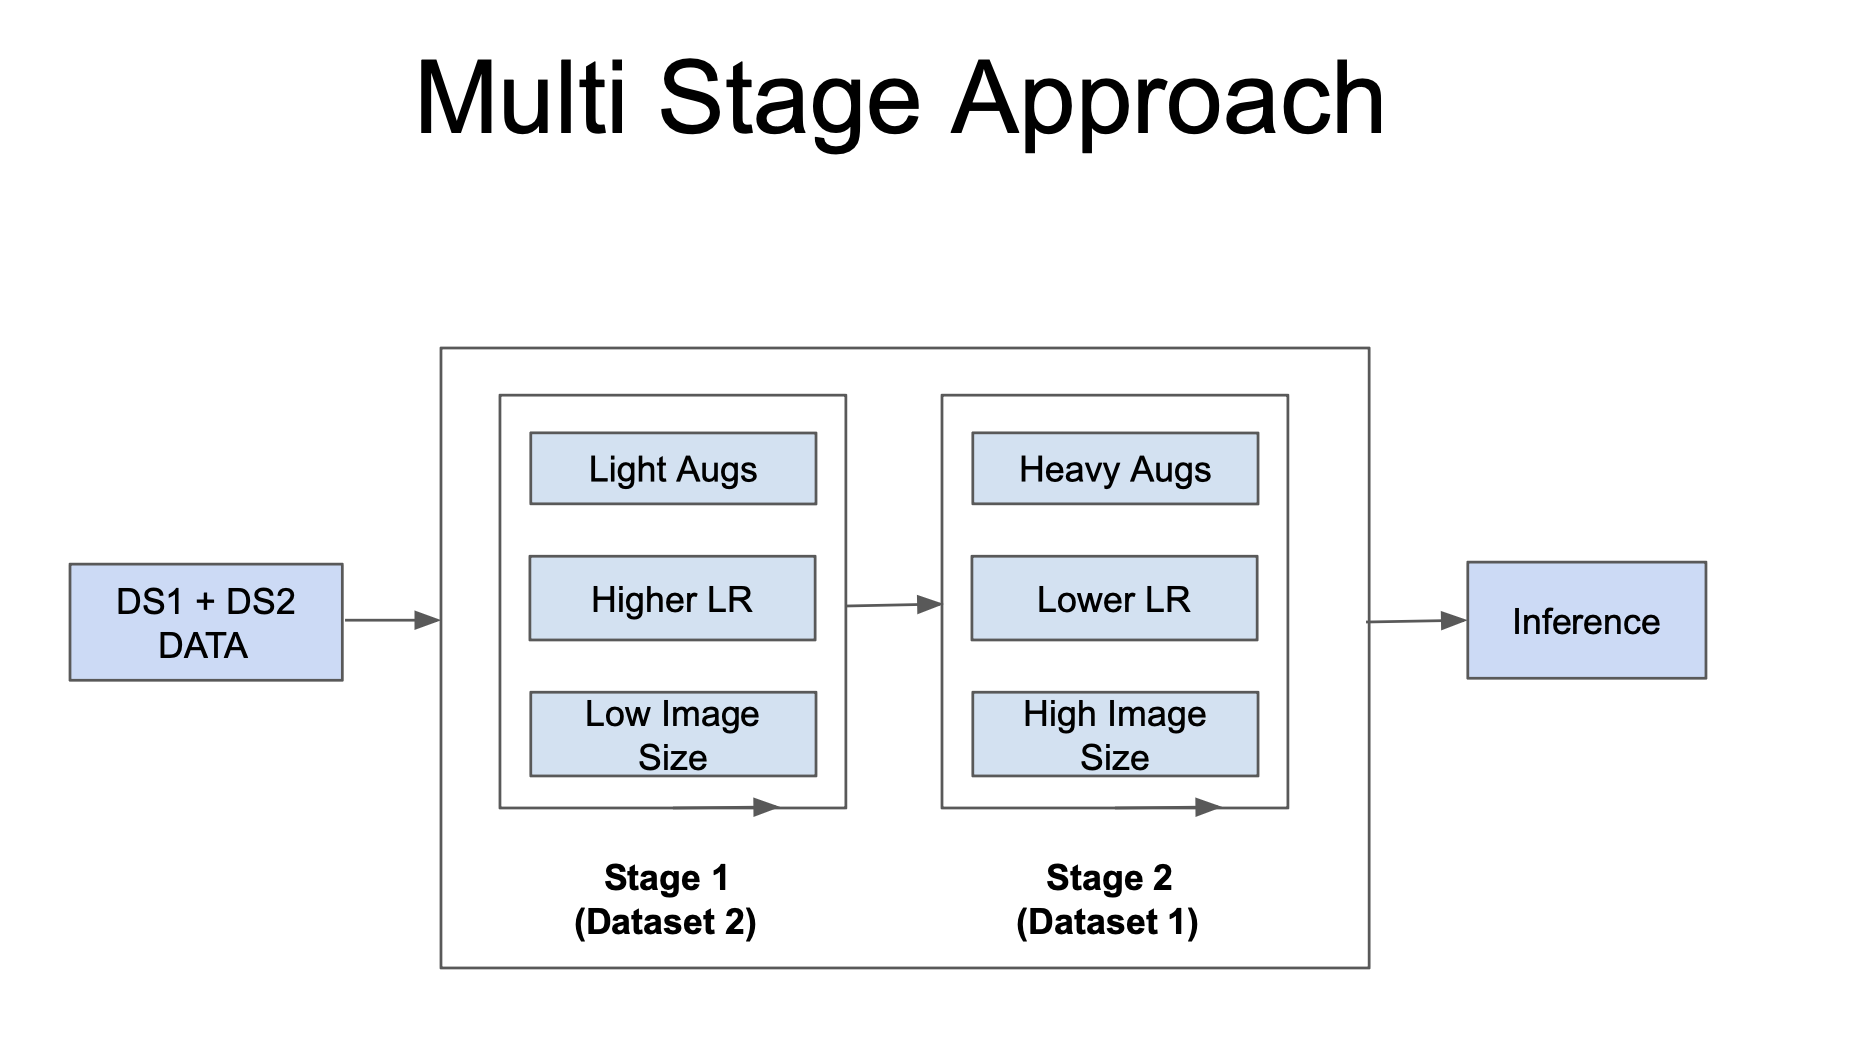
\includegraphics[width=0.98\linewidth]{figure/third_place_multistage.png}
    \caption{Third-place multi-stage training diagram from the Kaggle write-up~\cite{nischay2023hubmapthird}. The central idea is to use Dataset 2 for broad noisy pretraining and Dataset 1 for clean high-resolution fine-tuning.}
    \label{fig:third_multistage}
\end{figure}

The same write-up also describes a pseudo-label extension for Dataset 3. In that branch, multi-stage models generate predictions, WBF ensembles them, confidence thresholding filters them, and the remaining pseudo labels are combined with Dataset 3 before another multi-stage training pass. The author states that pseudo labels were used in some final ensemble models, although they did not clearly improve leaderboard score. Reported useful techniques include multi-stage training, flip TTA, higher mask-head loss weights for HTC-based models, SGD, WBF, and erosion followed by one dilation step as post-processing.

\begin{figure}[H]
    \centering
    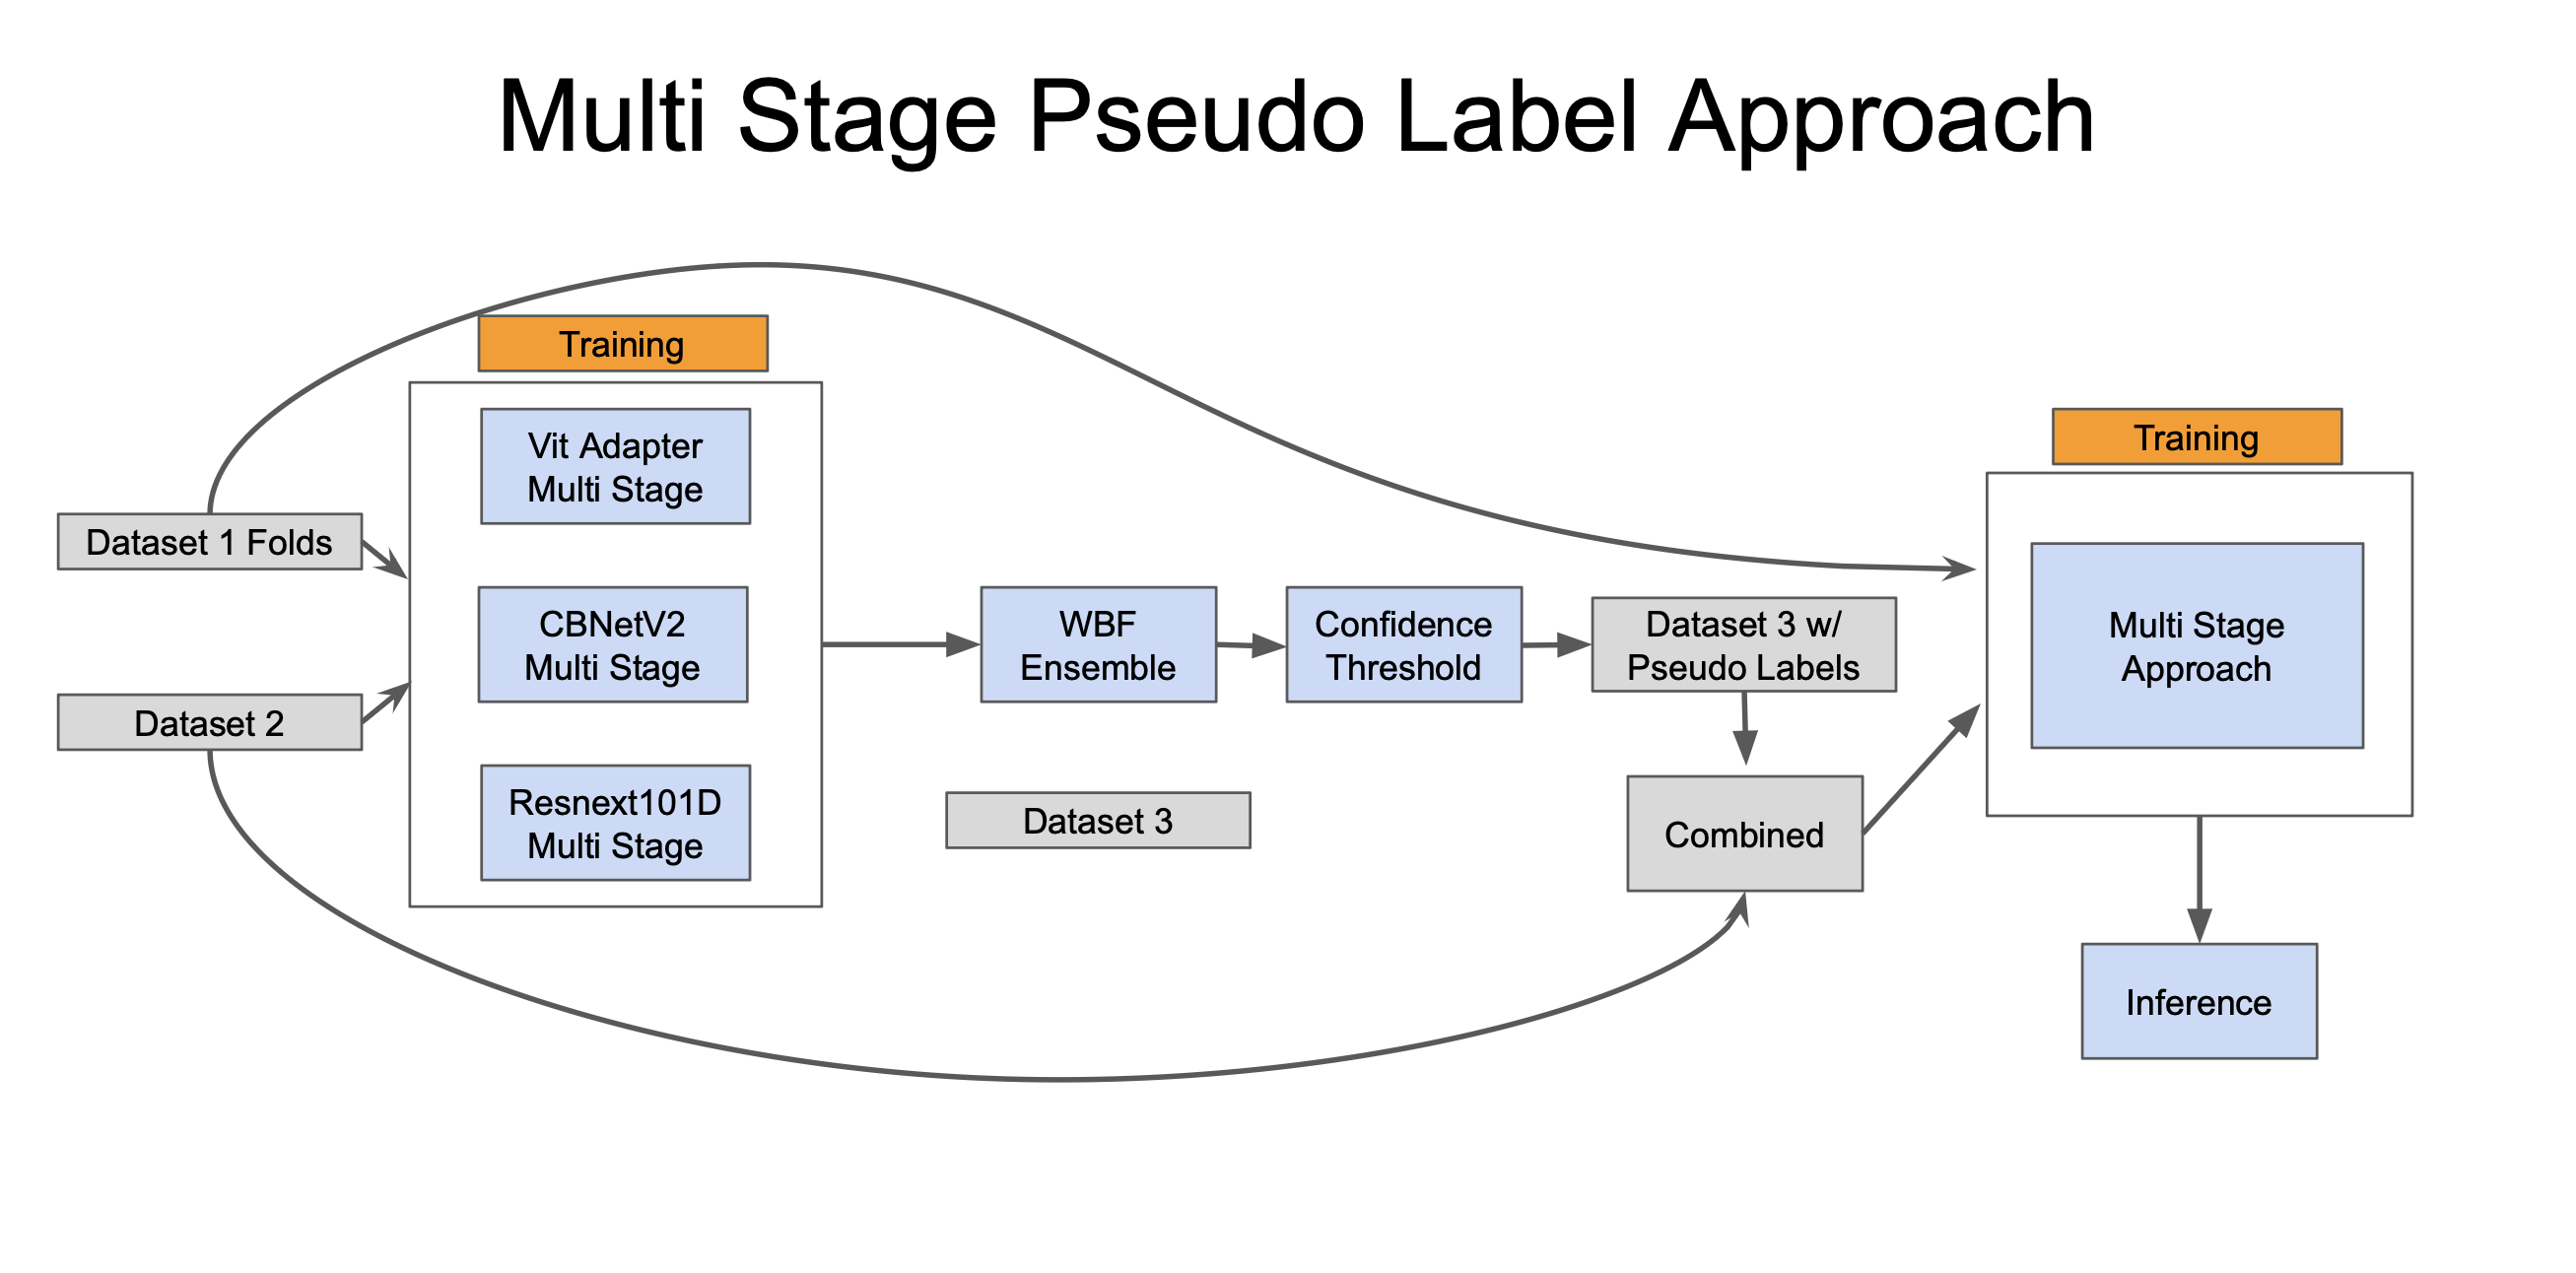
\includegraphics[width=0.98\linewidth]{figure/third_place_pseudo_label.png}
    \caption{Third-place pseudo-label extension from the Kaggle write-up~\cite{nischay2023hubmapthird}. Ensemble predictions are thresholded into Dataset 3 pseudo labels and then folded back into another multi-stage training pass.}
    \label{fig:third_pseudo}
\end{figure}

In our code this appears in \texttt{mmdet\_v3\_solution}: Stage 1 trains on Dataset 2, and Stage 2 fine-tunes on Dataset 1. This strategy is reasonable because Dataset 2 can teach broad morphological priors, while Dataset 1 should correct boundary precision and class noise. However, the original third-place system used much larger high-capacity backbones, higher training and inference resolutions such as 1400--2048 pixels, multi-scale inference, and a five-model ensemble. Our experiment replaces that family with an InternImage-T backbone inside Cascade Mask R-CNN. This makes the experiment informative but not a faithful reproduction of the third-place architecture.

\section{Experiment 1: First-place direction --- adding a YOLO26-Seg stream}
\label{sec:yolo}

\subsection{Motivation}

The first experiment asks whether adding a modern YOLO segmentation model can improve the first-place ensemble. The hypothesis is straightforward: YOLO26-Seg is architecturally different from Cascade/Mask R-CNN style models, so it may add useful diversity. If its errors are complementary, WBF should produce better boxes and therefore better final masks.

\subsection{Reproduced first-place ensemble baseline}

The first-place pipeline is the baseline we extend. Its inference notebook runs ten MMDetection streams:
\[
\{\texttt{r0i}, \texttt{r1i}, \texttt{s0i}, \texttt{s1i}, \texttt{m0i}, \texttt{m1i}, \texttt{y0i}, \texttt{y1i}, \texttt{sb0i}, \texttt{sb1i}\}.
\]
Each stream outputs bounding boxes, scores, and labels, which are fused by Weighted Boxes Fusion (WBF)~\cite{wbf}. The fused boxes are then passed into a Mask R-CNN style mask branch from \texttt{m1i} to produce final instance masks at input size $1440$. The original first-place author reported 0.589 private and 0.317 public. Our closest first-place-only rerun used the released first-place models with TTA and scored 0.577 private and 0.316 public, so the reproduction is essentially on par on public but about 0.012 lower on private.

\subsection{Data processing}

For YOLO experiments we use a dedicated preprocessing pipeline. Each $512 \times 512$ tile is padded to $768 \times 768$ by stitching neighboring tiles when available, and neighbor polygons are shifted into the padded coordinate frame, which reduces truncation artifacts for vessels crossing tile boundaries. The output is written in Ultralytics YOLO segmentation format with four spatial folds. The split uses Dataset 1 for validation and excludes spatially overlapping Dataset 2 tiles from the corresponding training fold to reduce leakage.

\subsection{Method}

We trained a four-fold YOLO26x-Seg ensemble using Ultralytics. The training script uses:
\begin{itemize}
    \item input size $768 \times 768$, matching the padded tile size;
    \item AdamW with fixed learning rate $10^{-3}$;
    \item heavy geometric augmentation: $180^\circ$ rotation, flips, scale, mosaic, mixup, and copy-paste;
    \item class filtering at inference so that only \texttt{blood\_vessel} instances are submitted.
\end{itemize}

The YOLO stream is inserted into the original notebook between the MMDetection inference cells and the WBF cell. Each YOLO fold produces \texttt{yolo0.pkl} to \texttt{yolo3.pkl}, using the same dictionary format as MMDetection:
\[
\texttt{pred\_instances} = \{\texttt{bboxes}, \texttt{scores}, \texttt{labels}\}.
\]
This makes YOLO a drop-in WBF stream. In the modified WBF cell, the four YOLO streams are assigned weights \([2,2,2,2]\) and can be enabled with \texttt{ABLATION\_MODE = baseline}.

\subsection{Results and analysis}

The YOLO-only validation results were reasonable for a lightweight independent stream, but they did not beat the reproduced first-place ensemble on private leaderboard. The best local fold-level YOLO mask mAP@50:95 ranged from 0.137 to 0.215, as shown in Table~\ref{tab:yolo_folds}. The full Kaggle submission records are summarized in Table~\ref{tab:kaggle_submissions}.

\begin{table}[H]
    \centering
    \small
    \begin{tabular}{lccc}
        \toprule
        Fold & Best epoch & Mask mAP@50 & Mask mAP@50:95 \\
        \midrule
        0 & 76 & 0.226 & 0.137 \\
        1 & 59 & 0.255 & 0.160 \\
        2 & 76 & 0.305 & 0.215 \\
        3 & 59 & 0.302 & 0.203 \\
        \bottomrule
    \end{tabular}
    \caption{Best local validation metrics of the YOLO26x-Seg folds from \texttt{runs/seg/fold*/results.csv}.}
    \label{tab:yolo_folds}
\end{table}

\begin{table}[H]
    \centering
    \scriptsize
    \begin{adjustbox}{width=\linewidth}
    \begin{tabular}{p{0.34\linewidth}p{0.43\linewidth}cc}
        \toprule
        Submission setting & Inference / fusion details & Private & Public \\
        \midrule
        Original first-place author & Public Kaggle write-up score & 0.589 & 0.317 \\
        First-place models only & Released first-place models with TTA inference & 0.577 & 0.316 \\
        YOLO26-Seg only & Four-fold YOLO26, direct inference, ensemble mask-NMS & 0.420 & 0.387 \\
        YOLO26-Seg only & Four-fold YOLO26, 4-way TTA \{\texttt{orig}, \texttt{hflip}, \texttt{vflip}, \texttt{rot90}\}, WBF and weighted mask average & 0.515 & 0.446 \\
        YOLO26-Seg + MedSAM-2 & YOLO prompts with MedSAM-2 LoRA and vendored MedSAM2 & 0.258 & 0.287 \\
        First-place + YOLO26-Seg & 10 first-place streams plus 4 YOLO streams, WBF weights \([2,2,2,2,1,1,1,1,2,2,2,2,2,2]\) & 0.572 & 0.304 \\
        First-place + YOLO26-Seg & Same 14-stream WBF with YOLO weights reduced to \([0.5,0.5,0.5,0.5]\) for the last four streams & 0.563 & 0.308 \\
        First-place + YOLO26-Seg & Explicit \texttt{streams=14} implementation with YOLO weights \([2,2,2,2]\) & 0.572 & 0.304 \\
        \bottomrule
    \end{tabular}
    \end{adjustbox}
    \caption{Kaggle submission scores from the tested inference variants.}
    \label{tab:kaggle_submissions}
\end{table}

\begin{figure}[H]
    \centering
    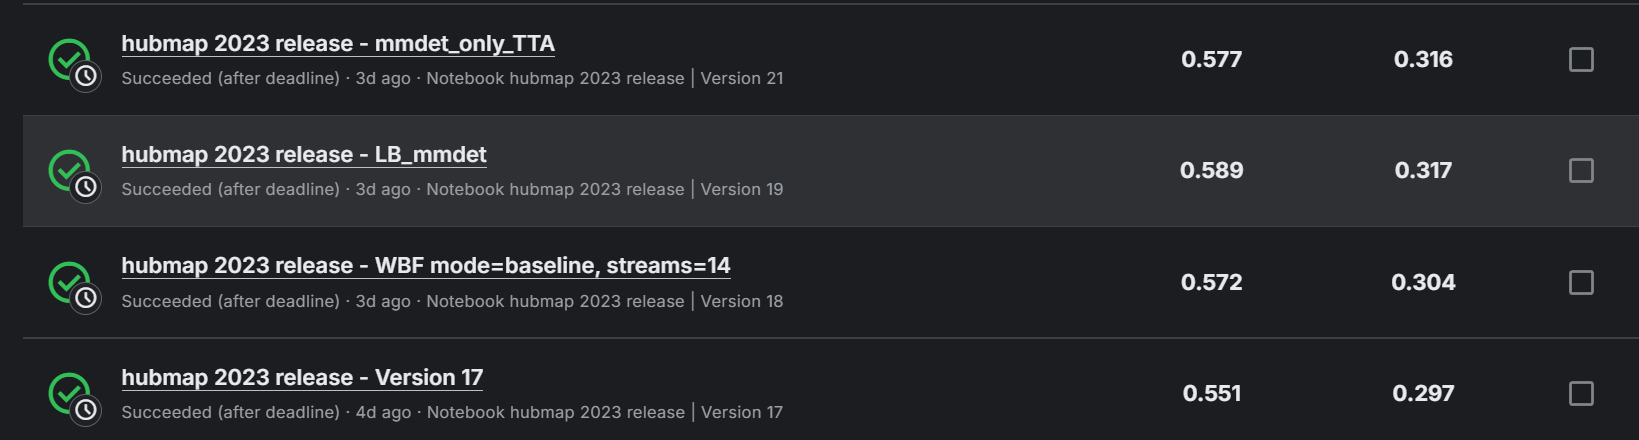
\includegraphics[width=0.98\linewidth]{figure/competition_exp1_score.png}
    \caption{Kaggle submission scores from the tested inference variants.}
    \label{fig:competition_score}
\end{figure}

These records clarify the gap between the experiments and the earlier report draft. YOLO26-Seg improved strongly when moving from direct mask-NMS to 4-way TTA with WBF and weighted mask averaging, rising from 0.420 to 0.515 private. However, adding YOLO streams into the first-place WBF did not improve the first-place system: the best 14-stream result was 0.572 private, below both our first-place-only TTA rerun at 0.577 and the author's 0.589. Lowering YOLO weights to 0.5 improved public score slightly but reduced private score to 0.563. The MedSAM-2 refinement branch also underperformed at 0.258 private, suggesting that prompt-driven mask refinement was not robust to the YOLO box distribution in this setup.

The negative result is still useful. First, YOLO did not provide enough diversity: many mistakes overlapped with the existing detector ensemble, especially on ambiguous vessel-like structures. Second, its bounding boxes were not consistently better than the Cascade/Mask R-CNN family. Since the final pipeline re-predicts masks from fused boxes, box quality dominates the final mAP. Third, the YOLO-only WBF/TTA variant looked attractive on public score (0.446 versus 0.316 for our first-place-only TTA rerun), but it was still weaker on private score (0.515 versus 0.577). Therefore, the public leaderboard alone was not reliable for selecting the final system, and adding a segmentation stream is not sufficient; the stream must improve private-set localization diversity.

\section{Experiment 2: Third-place direction --- two-stage InternImage Cascade}
\label{sec:internimage}

\subsection{Motivation}

The second experiment follows the multi-stage idea from high-ranking solutions: first learn from the larger noisy Dataset 2, then fine-tune on the cleaner Dataset 1. Instead of reproducing the original large ViT/CBNet/DetectoRS-style system, we implemented a more practical MMDetection v3 model that can run in our environment and be packaged for Kaggle.

\subsection{Data processing}

Annotations are converted from \texttt{polygons.jsonl} to COCO format. Dataset 1 is split spatially within WSI 1 and WSI 2 to create \texttt{dtrain0i.json} (train) and \texttt{dval0i.json} (validation), reusing the first-place \texttt{i} split, while Dataset 2 is exported as \texttt{dtrain\_\allowbreak dataset2.json} for the Stage 1 pretraining.

\subsection{Method}

The model is Cascade Mask R-CNN~\cite{cascade_rcnn} with:
\begin{itemize}
    \item \textbf{Backbone:} InternImage-T with pure PyTorch DCNv3 operators;
    \item \textbf{Neck:} FPN for multi-scale feature fusion;
    \item \textbf{Head:} 3-stage Cascade RoI head with progressively stricter IoU thresholds;
    \item \textbf{Mask branch:} FCN mask head with mask loss weight increased to 2.0;
    \item \textbf{Resolution:} $1024 \times 1024$ training images.
\end{itemize}

Stage 1 trains on \texttt{dtrain\_dataset2.json} for 10 epochs with light augmentation and AdamW learning rate $2 \times 10^{-4}$. Stage 2 loads the best Stage 1 checkpoint and fine-tunes on \texttt{dtrain0i.json} for 20 epochs with stronger augmentation, including random flips, AutoAugment color/geometric policies, and Albumentations elastic transform. The Kaggle inference package uses FP16, six-view TTA, morphological post-processing, and offline MMDetection dependencies.

The third-place write-up specifies a light and a heavy augmentation profile. The light profile (Stage 1) is \texttt{RandomFlip} (horizontal/vertical) plus an \texttt{AutoAugment} set of Shear, Translate, and Color$+$Equalize policies, followed by an Albumentations \texttt{ShiftScaleRotate}. The heavy profile (Stage 2) keeps these and adds \texttt{PhotoMetricDistortion}, \texttt{MinIoURandomCrop}, \texttt{CutOut}, and an Albumentations block of \texttt{RandomRotate90} with a \texttt{OneOf} over \texttt{ElasticTransform}, \texttt{GridDistortion}, and \texttt{OpticalDistortion}. Our implementation keeps the same light-then-heavy split but uses a simplified heavy profile --- \texttt{RandomFlip}, \texttt{AutoAugment} (color and geometric), and an Albumentations \texttt{RandomRotate90}$+$\texttt{ElasticTransform} --- and omits \texttt{CutOut}, \texttt{MinIoURandomCrop}, \texttt{GridDistortion}, and \texttt{OpticalDistortion}, which keeps the pipeline light enough for our single-GPU budget.

\subsection{Results and analysis}

Stage 1 reached local \texttt{coco/segm\_mAP} 0.130 at epoch 8 on \texttt{dval0i}. After fine-tuning on Dataset 1, Stage 2 improved substantially and reached 0.440 local \texttt{coco/segm\_mAP} at epoch 12. This confirms that the Dataset2 $\rightarrow$ Dataset1 schedule is useful. However, the result still did not surpass the reproduced first-place ensemble, and it is below what one would expect from a faithful third-place-style system.

\begin{table}[H]
    \centering
    \small
    \begin{tabular}{lcccc}
        \toprule
        Model / stage & Data & Best epoch & BBox mAP & Segm mAP \\
        \midrule
        InternImage Cascade Stage 1 & Dataset 2 & 8 & 0.181 & 0.130 \\
        InternImage Cascade Stage 2 & Dataset 1 & 12 & 0.407 & 0.440 \\
        \bottomrule
    \end{tabular}
    \caption{Local MMDetection validation metrics on \texttt{dval0i}. These are not directly comparable to Kaggle private leaderboard scores.}
    \label{tab:internimage}
\end{table}

We also packaged the Stage 2 checkpoint for Kaggle and submitted it with the FP16 / six-view-TTA / morphological pipeline. The submission score depends strongly on the detection score threshold, as shown in Figure~\ref{fig:competition_exp2_score}. Raising \texttt{--score-thr} to $0.3$ gave 0.372 private and 0.179 public, while lowering it to the code default of $0.001$ improved both to 0.395 private and 0.241 public. This matches the design note in \texttt{kaggle\_infer.py}: because the HuBMAP metric integrates average precision over the confidence ranking, discarding low-confidence detections early throws away recall that the AP integral would otherwise reward. A low threshold keeps the full ranked list and lets the metric, not a hard cutoff, decide where precision and recall trade off. The single-model InternImage stream therefore peaks at 0.395 private, which is consistent with its local segmentation mAP being far below the ten-stream first-place ensemble.

\begin{figure}[H]
    \centering
    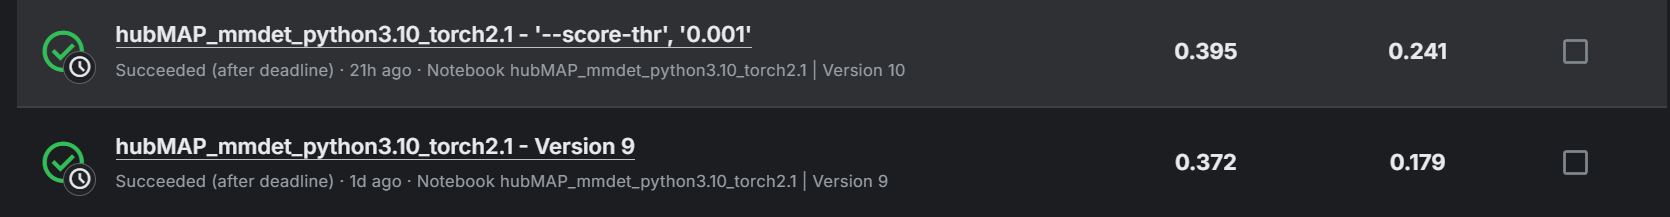
\includegraphics[width=0.98\linewidth]{figure/competition_exp2_score.png}
    \caption{Kaggle leaderboard scores of the two-stage InternImage-T Cascade Mask R-CNN, using FP16, six-view TTA, and morphological post-processing. Lowering the score threshold from $0.3$ to the code default $0.001$ improves both private and public scores.}
    \label{fig:competition_exp2_score}
\end{figure}

For reference, the third-place solution itself scored 0.583 private and 0.619 public~\cite{nischay2023hubmapthird}. The gap between its public and private scores is tiny, and even slightly reversed, in sharp contrast to the first place, whose public score ($0.317$) sits far below its private score ($0.589$). This points to much less distribution shift across the two leaderboard splits: because the third place's later stage still drew on the broad Dataset 2 (and Dataset 3) WSIs, the model generalizes almost identically to public and private tiles. Our two-stage InternImage-T inherits the same schedule but, with a far smaller backbone, a single stream, and lower resolution, peaks at 0.395 / 0.241 --- the multi-stage idea transfers, but the capacity does not.

The main reason it stays below the ensemble is architecture mismatch. The referenced multi-stage solution direction relies on very large transformer-style backbones and detector ensembles. Our InternImage-T model is much smaller and is a different system. A second reason is Dataset 2 noise: a compact model may absorb noisy masks more directly, whereas a larger pretrained backbone can be more robust. Finally, our implementation used only a single InternImage Cascade stream. The first-place baseline derives much of its strength from ensembling and from using a dedicated high-resolution mask re-prediction stage.

\section{Discussion}
\label{sec:discussion}

The two experiments show that leaderboard-level instance segmentation is a systems problem, not only a model-choice problem. The first-place pipeline works because it separates responsibilities: many models propose boxes, WBF filters and averages localization evidence, and a strong mask branch converts fused boxes into final masks. This structure also explains why the YOLO experiment did not help the final ensemble. YOLO26-Seg produced a reasonable standalone result after WBF/TTA (0.515 private, 0.446 public), but adding it to the first-place streams reduced the private score from our first-place-only 0.577 to 0.572.

The InternImage experiment gives a different lesson. Multi-stage training is useful: Stage 2 improved the local segmentation mAP from 0.130 to 0.440, and on Kaggle the single stream reached 0.395 private / 0.241 public once the score threshold was kept low. But borrowing only the training schedule is not enough to reproduce a top solution. Backbone capacity, resolution, label-noise robustness, and ensemble integration all interact. InternImage-T was attractive because it was easier to package and run, especially with a pure PyTorch DCNv3 implementation, but this practical choice also limited its ceiling.

Overall, our best direction remains the reproduced first-place MMDetection ensemble. The YOLO and InternImage experiments are valuable ablations: YOLO tested whether simple diversity improves WBF, while InternImage tested whether Dataset2 pretraining transfers to Dataset1 fine-tuning. The submission gap is now clear: the original author reported 0.589 private, our first-place-only TTA rerun reached 0.577, and the best YOLO-augmented first-place ensemble reached 0.572. Future improvements should therefore focus on better box proposals, higher-capacity backbones, stronger WSI-aware validation, and more careful fusion rather than simply adding more segmentation outputs.

\section{Conclusion}
\label{sec:conclusion}

We reproduced the structure of the HuBMAP first-place solution and explored two extensions. The original first-place score was 0.589 private / 0.317 public, while our first-place-only TTA rerun reached 0.577 / 0.316. YOLO26x-Seg alone improved from 0.420 / 0.387 with direct mask-NMS to 0.515 / 0.446 with 4-way TTA, WBF, and weighted mask averaging, but inserting YOLO into the first-place WBF reduced private score to 0.572. The YOLO + MedSAM-2 branch was worse at 0.258 / 0.287. A two-stage Cascade Mask R-CNN with InternImage-T confirmed the benefit of Dataset2 pretraining followed by Dataset1 fine-tuning, scoring 0.395 private / 0.241 public at a low score threshold (versus 0.372 / 0.179 at threshold 0.3), but the smaller backbone and single-model setup remained below the reproduced ensemble baseline. The project therefore supports a central conclusion: for this competition, high-quality box localization and ensemble design are more important than mask sharpness alone.


\bibliographystyle{unsrt}
\bibliography{references}
\endgroup

\end{document}
